\documentclass[t]{beamer}
\usepackage{CJKutf8}
\usepackage{amsfonts}
    \usepackage{amsmath}
    \usepackage{amssymb}
    \usepackage{amsthm}
    \usepackage{enumerate}
    \usepackage{graphicx}
    \usepackage{layout}
    \usepackage{mathrsfs}
    \usepackage{fancyhdr}
    \usepackage{subfigure}
    \usepackage{tcolorbox}
    \usepackage{tikz-cd}
    \usepackage{color}
    \usepackage{pifont}
    \usepackage{verbatim}
    \usepackage{mathtools}
    \usepackage{float}
    \usepackage{bm}
    \usetheme{AnnArbor}
% \usetheme{Antibes}
\usecolortheme{beaver}
\usepackage{listings}

% 设置JSON样式
\lstdefinestyle{json}{
    basicstyle=\tiny\ttfamily,
    columns=fullflexible,
    showstringspaces=false,
    commentstyle=\color{gray},
    keywordstyle=\color{blue},
    stringstyle=\color{red},
    breaklines=true,
    frame=single,
    captionpos=b,
    aboveskip=10pt,
    belowskip=10pt
}

\lstset{
    language=Python, % 设置代码块语言为Python
    breaklines=true, % 自动换行
    basicstyle=\small\ttfamily, % 设置基本字体样式
    keywordstyle=\bfseries\color{blue}, % 设置关键字样式
    commentstyle=\itshape\color{gray}, % 设置注释样式
    showstringspaces=false, % 不显示字符串中的空格
    frame=single, % 设置代码块边框样式
    numbers=left, % 行号显示在左侧
    numberstyle=\tiny\color{gray}, % 设置行号样式
    stepnumber=1, % 设置行号间隔
    tabsize=4 % 设置制表符宽度
}


% 设置shell样式
\lstdefinestyle{shell}{
    language=bash,
    basicstyle=\tiny\ttfamily,
    columns=fullflexible,
    showstringspaces=false,
    commentstyle=\color{gray},
    keywordstyle=\color{blue},
    stringstyle=\color{red},
    breaklines=true,
    frame=single,
    captionpos=b,
    aboveskip=10pt,
    belowskip=10pt
}

% 添加网址的命令
\usepackage{hyperref}
% 这是一个带链接文本的示例:\href{https://www.example.com}{点击这里访问网站}
% 普通的示例:\url{https://www.example.com}
% 表格
\usepackage{booktabs}
\usepackage{multirow}

% \setbeamertemplate{navigation symbols}{}

\usepackage{textpos}

\newcommand{\dif}{\mathrm{d}}
\newtheorem{thm}{{定理}}

% some common command
\newcommand{\mm}[1]{$ #1$\newline}
% \newcommand{\tuichu}{\Rightarrow}
% \newcommand{\li}[1]{\newline#1}



\newcommand{\analysis}[2]{\forall \mathcal{E}{#1},\exists \delta {#2},s.t.}
\newcommand{\denyanalysis}[2]{\exists \mathcal{E}{#1},\forall \delta {#2},s.t.}
\newcommand{\yield}{\Rightarrow }
\newcommand{\jj}{\newline}
\newcommand{\ff}[1]{$ #1$}   % math environment + newline
\newcommand{\fgn}[1]{\begin{equation}#1\end{equation}  }
\newcommand{\fg}[1]{$$ #1$$}   % math environment + newline 
\newcommand{\pf}{$proof.$\newline}
\newcommand{\ee}{\newline\ff{\Box}\newline}
\newcommand{\fenshi}[2]{\ff{\frac{#1}{#2}}}
\newcommand{\shenlue}{\vdots\jj}
\newcommand{\abs}[1]{{\left \lvert #1 \right\rvert}}
\newcommand{\loge}[1]{In ({#1})}
\newcommand{\logical}[2]{log_{#2}^{#1}}
\newcommand{\summary}[3]{$\sum_{{#1}={#2}}^{#3}  $}
\newcommand{\denjia}[2]{{#1}\Leftrightarrow {#2}}
\newcommand{\jihe}[3]{ {#1}  = \{ {#2} \mid {#3} \} }
\newcommand{\ve}[2]{\left\langle {#1},{#2}\right \rangle}
\newcommand{\dakuohao}[2]{\begin{array}{rcl}{#1}\end{array} \} \Rightarrow{#2}}
\newcommand{\sxb}[3]{#1^{#2}_{#3}}
\newcommand{\sss}[2]{#1^{#2}}
\newcommand{\xxx}[2]{#1_{#2}}
\newcommand{\bri}[1]{\uppercase\expandafter{\romannumeral#1}}
\newcommand{\ri}[1]{\romannumeral#1} 
\newcommand{\polynomial}[8]{#1_{#2}#6^{#7}+#1_{#3}#6^{#8}+...+#1_{#4}#6+#1_{#5} }
\newcommand{\newd}[4]{f[{#1}_{#2},{#4},{#1}_{#3}]}
\newcommand{\lb}[2]{\begin{align*}\begin{split}{#1}\{ {#2}\end{split}\end{align*}}
\newcommand{\tab}[1]{\begin{array}{ll} {#1}\end{array}}


% 向量乘积
\newcommand{\avg}[1]{\left\langle #1 \right\rangle}
% 偏微分方程
\newcommand{\difFrac}[2]{\frac{\dif #1}{\dif #2}}
\newcommand{\pdfrac}[2]{\frac{\partial{#1}}{\partial{#2}}}
% 不同章节
\newcommand{\one}[1]{\section{#1}}
\newcommand{\two}[1]{\subsection{#1}}
\newcommand{\three}[1]{\subsubsection{#1}}
\newcommand{\aone}[1]{\section*{#1}}
\newcommand{\atwo}[1]{\subsection*{#1}}
\newcommand{\athree}[1]{\subsubsection*{#1}}
% 大括号,左右都有
\newcommand{\lbra}[1]{\left\{  {\begin{matrix} #1 \end{matrix}}\right. } 
% 样式 括号前缀 + 括号 
\newcommand{\lbras}[2]{{#1}\left\{ {  {\begin{matrix} #2 \end{matrix}}}\right. } 
\newcommand{\rbra}[1]{ \left.  {\begin{matrix} #1 \end{matrix}} \right\}  } 
% 模长
\newcommand{\distance}[1]{\parallel #1\parallel }
% 等价
\newcommand{\equ}{\Longleftrightarrow }
% 共轭
\newcommand{\cja}[1]{\overline{#1}}
% 两个矩阵,上面是 方框[] 下面是线条| 中间是 无
\newcommand{\mtx}[1]{\begin{matrix}#1\end{matrix} }
\newcommand{\bmtx}[1]{\begin{bmatrix}#1\end{bmatrix} }
\newcommand{\vmtx}[1]{\begin{vmatrix}#1\end{vmatrix} }
% \newcommand{\table}[1]{\begin{array}[lr]{ccc} #1 \end{array}}

%输入普通字符
\newcommand{\ww}[1]{\text{#1}}

% 所有内容 直接头文件搞定
\newcommand{\everything}[1]{\begin{document}\begin{CJK*}{UTF8}{gkai}#1\end{CJK*}\end{document}}


% 存放代码(失败了)
\newcommand{\cccode}[1]{\begin{lstlisting}#1\end{lstlisting}}

% 改变特定行序列
\newcommand{\ttt}{\subsection{}}

% 嵌套序号
\newcommand{\eee}[1]{\begin{enumerate}#1\end{enumerate}}


% 模板里面的一些宏
\newcommand{\pdfFrac}[2]{\frac{\partial #1}{\partial #2}}
\newcommand{\OFL}{\mathrm{OFL}}
\newcommand{\UFL}{\mathrm{UFL}}
\newcommand{\fl}{\mathrm{fl}}
\newcommand{\op}{\odot}
\newcommand{\Eabs}{E_{\mathrm{abs}}}
\newcommand{\Erel}{E_{\mathrm{rel}}}
% 变化颜色
\newcommand{\red}{\textcolor{red}}
\newcommand{\blue}{\textcolor{blue}}



% 流程图需要用到的宏包
\usepackage{palatino}
\usepackage{tikz}
\usetikzlibrary{shapes.geometric, arrows}
\tikzstyle{startstop} = [rectangle, rounded corners, minimum width = 2cm, minimum height=1cm,text centered, draw = black, fill = red!40]
\tikzstyle{io} = [trapezium, trapezium left angle=70, trapezium right angle=110, minimum width=2cm, minimum height=1cm, text centered, draw=black, fill = blue!40]
\tikzstyle{process} = [rectangle, minimum width=3cm, minimum height=1cm, text centered, draw=black, fill = yellow!50]
\tikzstyle{decision} = [diamond, aspect = 3, text centered, draw=black, fill = green!30]
% 箭头形式
\tikzstyle{arrow} = [->,>=stealth]
% 4个非常重要 的新命令
\newcommand{\start}[2]{    \node (start) [startstop]{#1};\node (in1) [io, below of = start]{#2};\lin{start}{in1}{}}
\newcommand{\stopp}[3]{\node (out1) [io, below of= #1]{#2};\node (stop) [startstop, below of=out1]{#3};\lin{out1}{stop}{} }
\newcommand{\pro}[6]{    \node (#3) [process, #2 of=#1,xshift=#4 cm]{#5};}
\newpage
\newcommand{\lin}[3]{\draw [arrow] (#1) --node [above] {#3} (#2);}


\begin{document}
\begin{CJK*}{UTF8}{gkai}
% 一般第一页显示PPT标题以及作者信息

% \BackgroundPic{./Screenshot from 2022-04-20 16-31-08.png}

% 增加学校 前面
\addtobeamertemplate{title page}{}{
	\begin{tikzpicture}[remember picture,overlay]
		% \node[yshift=85pt,xshift=50pt]{\includegraphics[height=2cm]{Screenshot from 2022-04-20 16-51-21.png}};
\end{tikzpicture}
}


	% \title{时间序列数据集}
	\title{组会汇报}
	\subtitle {} %不需要
	\author{
		陈钶杰\, \\
		专业:计算数学\,
	} % 显示作者
	% \institute {学院:数学科学学院} % 设置学院机构	
	\date{\today}  % 显示日期
\titlepage

% 设置目录
\begin{frame}{目录}
\frametitle{目录}	
\tableofcontents  % 显示目录
\end{frame} 


\section{模型运行结果}



\subsection{预测结果展示}

\begin{frame}
	\frametitle{\small 总数据量:10000,8预测4,短向量序列预测}	
	\begin{itemize}
		\item 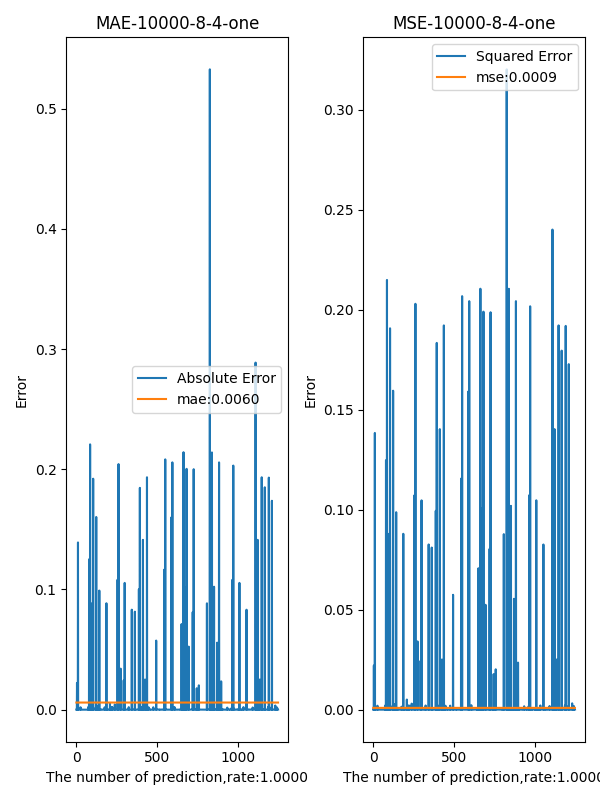
\includegraphics[scale=0.371]{png/10000-8-4-one.png}
	\end{itemize}
\end{frame}

\begin{frame}
	\frametitle{\small 总数据量:30000,8预测4,短向量序列预测}	
	\begin{itemize}
		\item 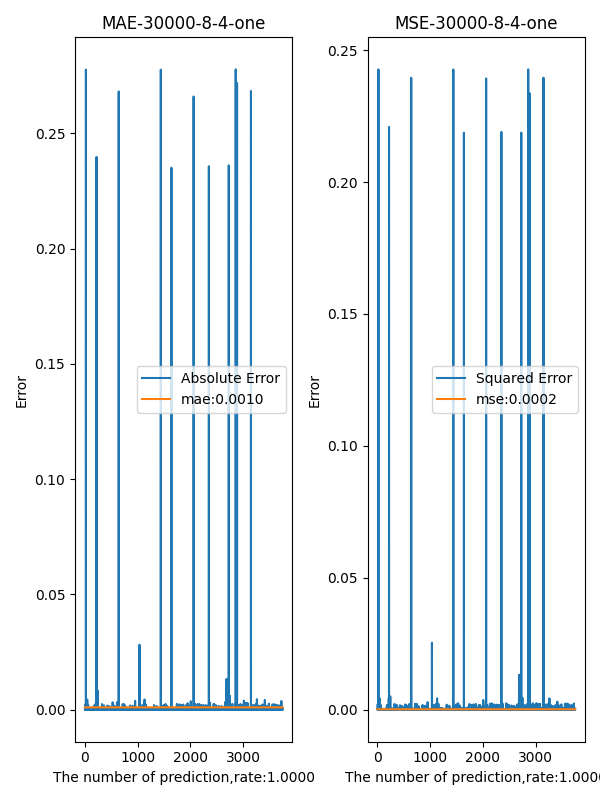
\includegraphics[scale=0.371]{png/30000-8-4-one.png}
	\end{itemize}
\end{frame}

\begin{frame}
	\frametitle{\small 总数据量:30000,16预测8,短向量序列预测}	
	\begin{itemize}
		\item 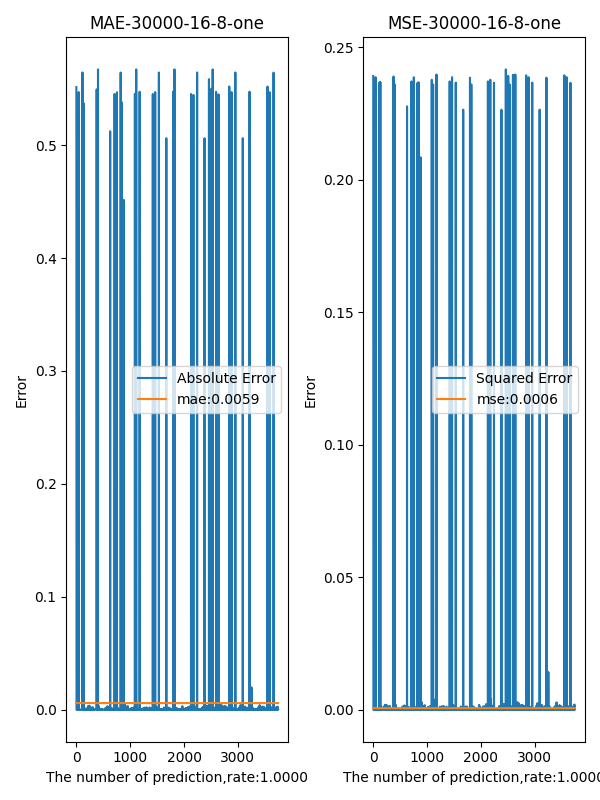
\includegraphics[scale=0.371]{png/30000-16-8-one.png}
	\end{itemize}
\end{frame}

\begin{frame}
	\frametitle{\small 总数据量:30000,16预测8,长向量序列预测}	
	\begin{itemize}
		\item 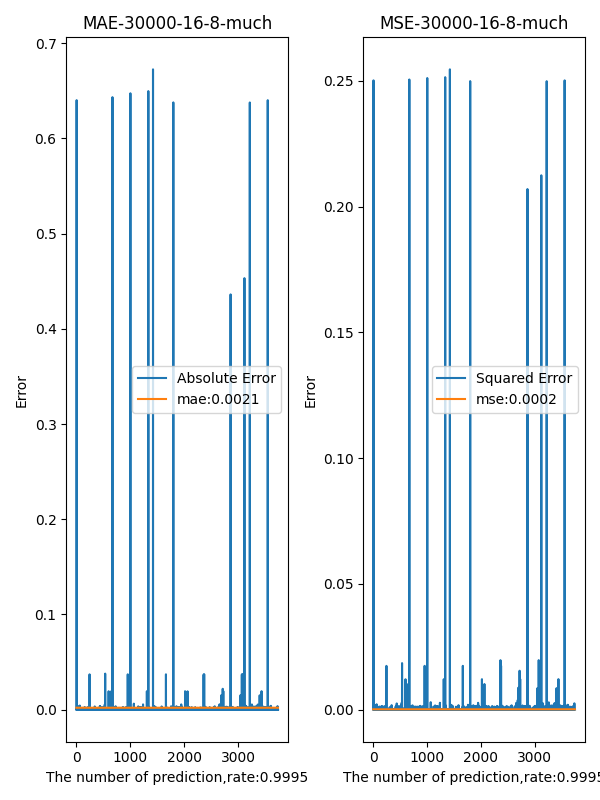
\includegraphics[scale=0.371]{png/30000-16-8-much.png}
	\end{itemize}
\end{frame}

% \begin{frame}
% 	\frametitle{\small 总数据量:30000,8预测4,多序列预测}	
% 	\begin{itemize}
% 		\item 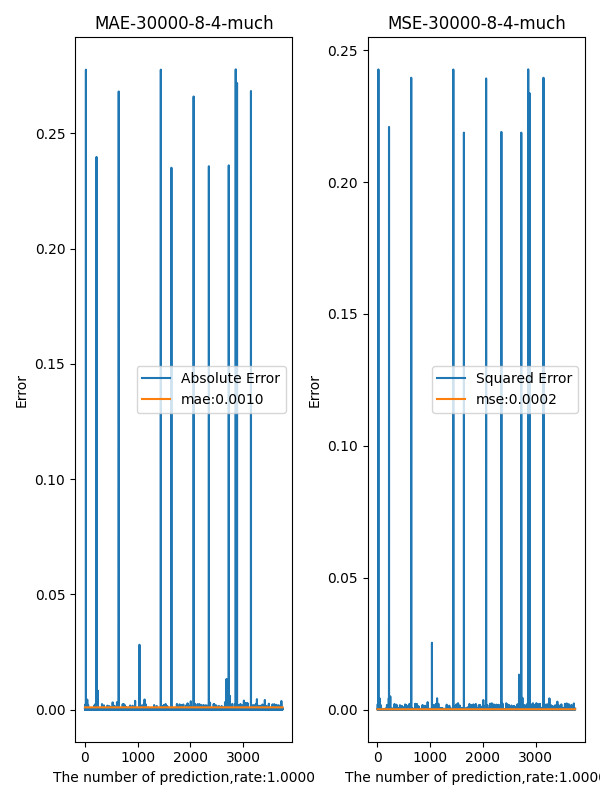
\includegraphics[scale=0.371]{png/30000-8-4-much.png}
% 	\end{itemize}
% \end{frame}

\begin{frame}
	\frametitle{\small 总数据量:20000,16预测8 和 8预测4,短向量序列预测}	
	\begin{itemize}
		\item 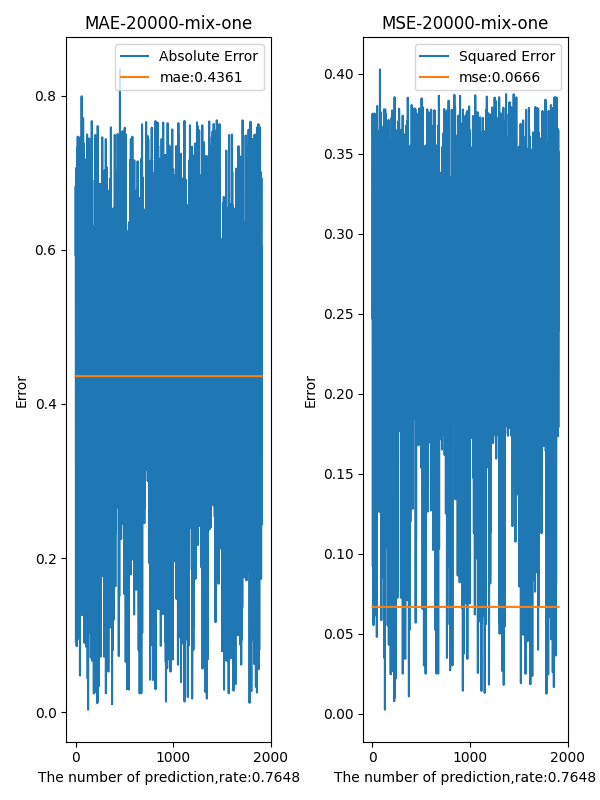
\includegraphics[scale=0.371]{png/20000-mix-one.png}
	\end{itemize}
\end{frame}

\begin{frame}
	\frametitle{\small 总数据量:40000,16预测8 和 8预测4,混合长短向量序列预测}	
	\begin{itemize}
		\item 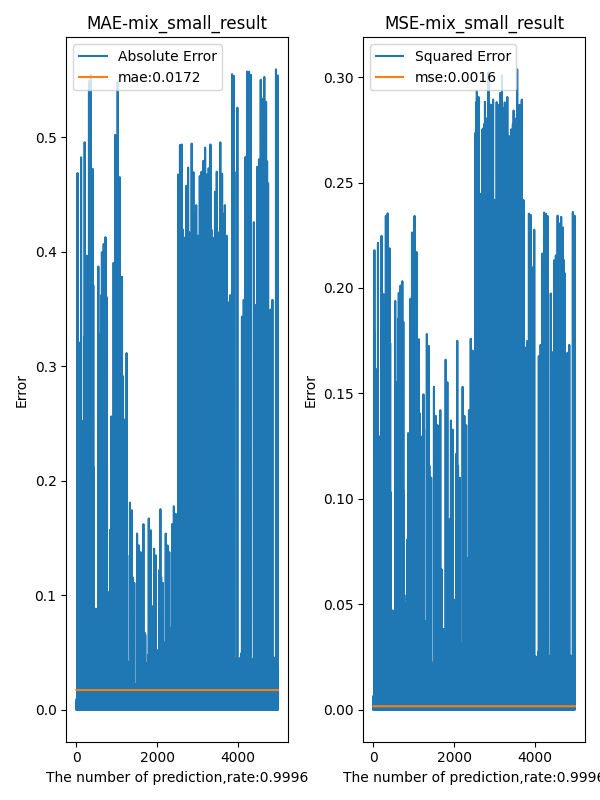
\includegraphics[scale=0.371]{png/mix_small_result.png}
	\end{itemize}
\end{frame}

\begin{frame}
	\frametitle{\small 总数据量:120000,16预测8 和 8预测4,混合长短向量序列预测}	
	\begin{itemize}
		\item 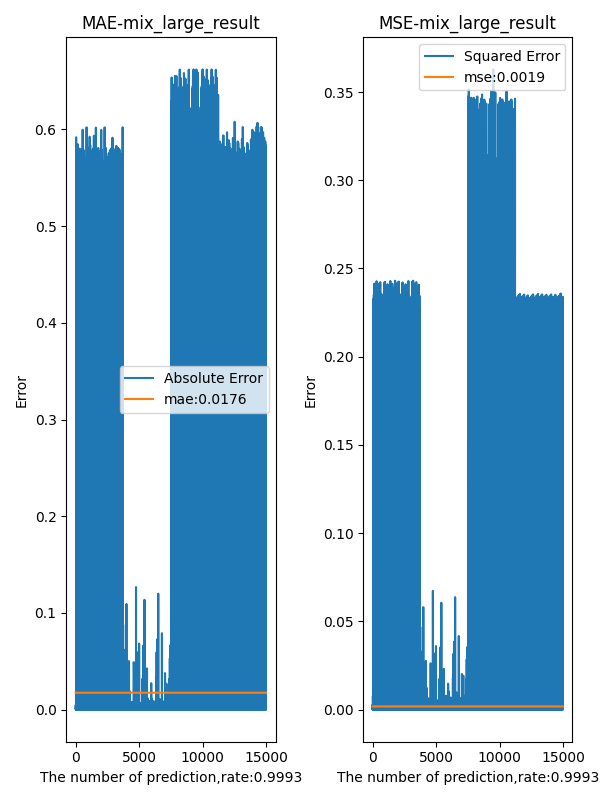
\includegraphics[scale=0.371]{png/mix_large_result.png}
	\end{itemize}
\end{frame}


\subsection{实验结果分析}
\begin{frame}
	\frametitle{根据数据的结论}	
	\begin{itemize}
		\item 当预测任务,以及预测序列相同时,可以看出给定训练的序列越长,效果越好。
		\item 当训练数据集的数量,测试的序列相同时,预测的长度越短,效果越好。
		\item 当训练总数据集数量,预测长度相同时,训练的序列向量越长,对最终的预测结果更加精确。
		\item 对于一个预测长度不一致的数据集合,最终的误差比较大,且预测序列长度和目标序列长度相似度大约是76\%
		\item 从混合的预测长度,时间序列的数据集合训练结果中也可以看出这个长向量时间序列的预测结果要好于短向量的结果,且预测短的序列要优于预测长序列的误差。
		% \item 8-4 one  8-4  much  16-8 one 16-8 much
        % \item 
	\end{itemize}
\end{frame}


\subsection{实验过程中遇到的一些问题}

\begin{frame}
	\frametitle{遇到的问题}	
	\begin{itemize}
        \item 目标预测的个数和实际预测个数不同或者预测非数值形式,下面是一些解决方法
        \eee{
            \item 忽略实际预测个数和目标个数不同的例子,并计算其比率rate(目标与实际个数相同的个数/测试集个数)
            \item 对预测得到的结果进行截断或补零
        }   
        \item 序列长度太长的问题
	\end{itemize}
    % 目前考虑的是只考虑数量对等的
\end{frame}

\subsection{下一步的计划}
\begin{frame}
	\frametitle{实现目标}	
	\begin{itemize}
        \item 混合更多的元素,同时训练更多不同种类的时间序列和以及预测长度。
        \item 尝试对未见过的序列进行预测,看看结果如何。
        \item 提高模型参数精度,看看结果是否会有什么变化。        
        \item 开始对8个常见的时间序列进行测试。
	\end{itemize}
\end{frame}


% \subsection{图像结果展示}
% \subsection{测试的数据集}


\section{相关论文}
\begin{frame}
    \frametitle{prompt learning and time series论文(IEEE)}
\eee{
    \item 标题:Evaluating BERT on cloud-edge time series forecasting and sentiment analysis via prompt learning\\
    \item 结论:该论文使用即时学习评估了在云边缘时间序列预测和情感分析任务的大量数据上预训练的BERT的性能。实验结果表明,BERT在云边时间序列预测任务中表现不佳,这表明BERT没有良好的逻辑推理能力。选择均方误差 (MSE) 作为时间序列预测的评估指标,结果表明,使用即时学习的 BERT 无法根据前一个滑动窗口中的信息很好地预测下一个时间步长的特征。
}    



\end{frame}


% 结束语
\section{}
\begin{frame}
	\frametitle{}
	\begin{center}
		\Huge{谢谢老师和同学的聆听!}
	\end{center}
\end{frame}


\end{CJK*}
\end{document}